\section{Pengujian Prototipe \textit{High-Fidelity} Iterasi Pertama}
\label{sec:test_hifi_1}

Prototipe \textit{high-Fidelity} yang sudah dirancang perlu dilakukan pengujian. Pengujian dilakukan dengan menggunakan metode \textit{usability testing}. Pengujian prototipe \textit{low-fidelity} dilakukan untuk mengukur capaian dari tujuan-tujuan yang sudah ditentukan pada subbab \ref{subsec:analisis_goals}, yaitu \textit{usability goals} \textit{efficiency} dan \textit{learnability} serta \textit{user experience goals} \textit{helpful} dan \textit{motivating}. Untuk mengukur capaian-capaian tersebut, partisipan diminta untuk menyelesaikan beberapa \textit{task} terkait halaman, widget, dan fitur yang telah dirancang. Pada Tabel \ref{tab:daftar_pengujian_goals}, dilakukan pemetaan \textit{usability goals} dan \textit{user experience goals} dengan tujuan dan kriteria pengujian yang berkaitan.

\RaggedLeft
\begin{small}
\begin{longtable}[c]{|W{c}{0.16\textwidth}|>{\ccnormspacing}m{0.36\textwidth}|>{\ccnormspacing}m{0.36\textwidth}|}
  \caption{Pemetaan Tujuan dan Kriteria Pengujian terhadap \textit{Usability} dan \textit{User Experience Goals}}
  \label{tab:daftar_pengujian_goals} \\
  \hline \rowcolor[HTML]{A3E5F5}
  \textbf{Goals} & \multicolumn{1}{|c|}{\textbf{Tujuan Pengujian}} & \multicolumn{1}{|c|}{\textbf{Kriteria Pengujian}} \\ \hline \endfirsthead
  \hline \rowcolor[HTML]{A3E5F5}
  \textbf{Goals} & \multicolumn{1}{|c|}{\textbf{Tujuan Pengujian}} & \multicolumn{1}{|c|}{\textbf{Kriteria Pengujian}}\\ \hline \endhead
  \hline \endfoot

  % Usability Goals
  % \textit{Efficiency} & Mengukur seberapa efisien pengguna dalam melakukan aktivitasnya di dalam prototipe \textit{high-fidelity} & Mengukur waktu yang diperlukan dalam mengerjakan setiap \textit{task}, dan menggunakan kuesioner dari \textit{System Usability Scale} \\ \hline
  \textit{Efficiency} & Mengukur seberapa efisien pengguna dalam melakukan aktivitasnya di dalam prototipe \textit{high-fidelity} & Mengukur tingkat \textit{efficiency} aplikasi menggunakan kuesioner dari \textit{System Usability Scale} \\ \hline
  
  \textit{Learnability} & Mengukur seberapa mudah fitur-fitur aplikasi untuk dipelajari dan digunakan oleh pengguna & Mengukur tingkat kemudahan penggunaan aplikasi dengan \textit{Single Ease Question}\\ \hline
  
  % UX Goals
  \textit{Helpful} & Mengetahui apakah pengguna dapat merasa terbantu dalam melakukan aktivitasnya oleh fitur-fitur yang disediakan prototipe \textit{high-fidelity}  & Menggunakan skala \textit{value/usefulness} dari \textit{Intrinsic Motivation Inventory} untuk mengukur seberapa membantu aplikasi kepada pengguna \\ \hline
  
  \textit{Motivating} & Mengetahui apakah pengguna dapat merasa termotivasi untuk fokus pada pekerjaannya oleh fitur-fitur yang disediakan prototipe \textit{high-fidelity} & Menggunakan skala \textit{interest/enjoyment}, dan \textit{pressure/tension} dari \textit{Intrinsic Motivation Inventory} untuk mengukur tingkat motivasi pengguna setelah melakukan pengujian \\ \hline

\end{longtable}
\end{small}
\justifying
\FloatBarrier

\subsection{Langkah Pengujian}
\label{subsec:langkah_test_1}

Pengujian dilakukan dengan beberapa tahap, yaitu perkenalan, eksplorasi, pengerjaan \textit{task}, lalu diakhiri dengan penutupan. Rancangan pengujian yang lebih detail dapat dilihat pada Lampiran \ref{chpt:testing_hifi}. Berikut adalah penjelasan untuk setiap tahap pengujian

\begin{enumerate}
  \item Perkenalan
  \subitem Pada tahap ini, dilakukan perkenalan diri serta pengarahan singkat kepada partisipan. Pengarahan akan berisi pemaparan tentang prototipe yang akan diuji serta penjelasan terkait prosedur pengujian. 

  \item Eksplorasi
  \subitem Pada tahap ini, partisipan diberi kesempatan untuk melakukan eksplorasi terhadap prototipe yang akan diuji. Hal ini bertujuan agar partisipan memiliki wawasan yang cukup tentang aplikasi sebelum pengujian.

  \item Pengerjaan \textit{task}
  \subitem Pada tahap ini, partisipan mulai mengerjakan \textit{task-task} yang diberikan. Detail lebih lengkap dari task dapat dilihat pada Lampiran \ref{chpt:skenario_hifi1}. Setiap mengerjakan \textit{task}, kegiatan partisipan akan direkam waktunya sebagai bagian dari pengujian \textit{usability goal efficiency}. Selain itu, setiap kali partisipan selesai mengerjakan sebuah \textit{task}, mereka diminta untuk mengisi \textit{post-task questionnaire} yaitu \textit{Single Ease Question} (SEQ). SEQ menggunakan pertanyaan dengan jawaban \textit{likert-scale} untuk mengukur tingkat kemudahan penggunaan fitur dalam aplikasi.

  \item Pengisian \textit{post-test questionnaire}
  \subitem Pada tahap ini, partisipan telah selesai mengerjakan seluruh \textit{task} yang diberikan penguji. Partisipan akan diminta untuk mengisi \textit{post-test questionnaire} dalam bentuk \textit{System Usability Scale} (SUS) dan \textit{Intrinsic Motivation Inventory} (IMI). 

  \item Penutupan
  \subitem Pada tahap ini, pengujian diakhiri dengan penyampaian kesan pesan dari partisipan, serta ucapan terima kasih dari penguji. 

\end{enumerate}


\subsection{Hasil Pengujian Prototipe \textit{High-Fidelity} Iterasi Pertama}
\label{subsec:hasil_test_1}

Pengujian prototipe \textit{high-fidelity} iterasi pertama dilakukan dengan 5 (lima) orang, sesuai dengan perkataan dari \textcite{nielsenusabilityproblems} yang menyebutkan bahwa pengujian dengan 5 (lima) orang partisipan sudah cukup untuk menemukan rata-rata 85\% masalah dari desain, dalam hal ini prototipe \textit{high-fidelity}. Hasil pengujian lengkap dapat dilihat pada Lampiran \ref{chpt:hasil_test_hifi1}. Dari pengujian, didapatkan beberapa temuan penting dari partisipan tentang prototipe, yang rangkumannya dapat dilihat pada Tabel \ref{tab:daftar_temuan_hifi}


\RaggedLeft
\begin{small}
\begin{longtable}[c]{|W{c}{0.12\textwidth}|>{\ccnormspacingcenter}m{0.8\textwidth}|}
  \caption{Daftar Temuan Penting Pengujian Prototipe \textit{High-Fidelity} Iterasi Pertama}
  \label{tab:daftar_temuan_hifi} \\
  \hline \rowcolor[HTML]{A3E5F5}
  \textbf{Partisipan} & \textbf{Temuan Penting} \\ \hline \endfirsthead
  \hline \rowcolor[HTML]{A3E5F5}
  \textbf{Partisipan} & \textbf{Temuan Penting} \\ \hline \endhead
  \hline \endfoot

  1 & \cditem{
    \item Partisipan berekspektasi diberikan pengaturan \textit{default} Bedtime Mode berupa opsi jadwal
  } \\ \hline
    
  2 & \cditem{
    \item Partisipan merasa widget Dashboard memuat lebih dari 3 aplikasi teratas
    \item Partisipan merasa penjelasan pada halaman-halaman pengenalan fitur masih terlalu panjang
    } \\ \hline
    
  3 & \cditem{
    \item Partisipan merasa navigasi dari halaman Dashboard langsung ke App Timer tidak diperlukan dan cukup sulit dibedakan dengan navigasi ke halaman penggunaan aplikasi
  } \\ \hline
  
  4 & \cditem{
    \item Partisipan merasa memerlukan sebuah pesan pengingat sebelum mematikan Focus Mode atau App Timer untuk hari ini
    \item Partisipan merasa evaluasi Daily Goal sebaiknya tidak langsung muncul ketika selesai menentukan Daily Goal
  } \\ \hline
  
  5 & \cditem{
    \item Partisipan merasa penempatan fitur Smartphone Usage Evaluation kurang tepat pada halaman Daily Goal
    \item Partisipan merasa tombol + (plus) pada widget App Timer tidak diperlukan
  } \\ \hline

\end{longtable}
\end{small}
\justifying
\FloatBarrier

Berdasarkan temuan-temuan yang telah disebutkan di atas, maka disusun beberapa rencana perbaikan untuk direalisasikan dalam prototipe \textit{high-fidelity} iterasi kedua. Pada Tabel \ref{tab:daftar_perbaikan_hifi} dapat ditemukan daftar masalah yang disimpulkan dari temuan-temuan penting, beserta rencana perbaikan yang berkaitan.

\RaggedLeft
\begin{small}
\begin{longtable}[c]{|W{c}{0.05\textwidth}|>{\ccnormspacing}m{0.43\textwidth}|>{\ccnormspacing}m{0.43\textwidth}|}
  \caption{Daftar Rencana Perbaikan Prototipe \textit{High-Fidelity} Iterasi Pertama}
  \label{tab:daftar_perbaikan_hifi} \\
  \hline \rowcolor[HTML]{A3E5F5}
  \textbf{No} & \multicolumn{1}{|c|}{\textbf{Kesimpulan Masalah dari Temuan}} & \multicolumn{1}{|c|}{\textbf{Rencana Perbaikan}} \\ \hline \endfirsthead
  \hline \rowcolor[HTML]{A3E5F5}
  \textbf{No} & \multicolumn{1}{|c|}{\textbf{Kesimpulan Masalah dari Temuan}} & \multicolumn{1}{|c|}{\textbf{Rencana Perbaikan}}\\ \hline \endhead
  \hline \endfoot

  1 & Kurangnya opsi \textit{default} sebagai rekomendasi bagi pengguna untuk Bedtime Mode & Mengatur opsi \textit{default} pada Bedtime Mode menjadi Based on schedule \\ \hline
  2 & Kurangnya fungsionalitas dari widget Dashboard & Hal ini merupakan pilihan desain yang disengaja untuk mempertahankan kesederhanaan dari sebuah widget \\ \hline
  3 & Adanya navigasi ke halaman App Timer dari halaman Dashboard mengganggu navigasi ke halaman penggunaan aplikasi & Menghapus navigasi dari halaman Dashboard ke halaman App Timer \\ \hline
  4 & Kurangnya elemen yang menjaga pengguna dari kesalahan aksi pada fungsi yang cukup kritis & Menambahkan pesan pengingat untuk aksi yang cukup kritis seperti mematikan Focus Mode atau App Timer \\ \hline
  5 & Kurangnya penundaan waktu untuk memunculkan evaluasi dari penentuan Daily Goal pada halaman Daily Goal  & Menunda memunculkan evaluasi tepat setelah menentukan Daily Goal \\ \hline
  6 & Kurang tepatnya penempatan fitur Smartphone Usage Evaluation pada halaman Daily Goal & Menambahkan halaman khusus untuk memuat fungsi dari Smartphone Usage Evaluation \\ \hline
  7 & Tidak diperlukannya tombol penambahan App Timer untuk widget App Timer & Menghapus tombol penambahan App Timer dari widget App Timer \\ \hline
  
\end{longtable}
\end{small}
\justifying
\FloatBarrier

\newpage

\subsection{Analisis Hasil Pengujian Prototipe \textit{High-Fidelity} Iterasi Pertama}
\label{subsec:analisis_hasil_1}

Dari hasil pengujian pada prototipe \textit{high-fidelity} iterasi pertama, didapatkan beberapa skor dan temuan penting dari pengguna menurut kriteria-kriteria pengujian yang telah disebutkan pada Tabel \ref{tab:daftar_pengujian_goals}. Berikut adalah beberapa penjelasannya

\begin{enumerate}
  \item \textit{Single Ease Question} (SEQ)
  \subitem  Penilaian SEQ digunakan untuk mengetahui tingkat kemudahan sebuah \textit{task} untuk dapat diselesaikan oleh partisipan. Berdasarkan hasil nilai SEQ yang terdapat pada Gambar \ref{img:seq_1}, terlihat bahwa nilai yang diberikan setiap partisipan terhadap kemudahan pengerjaan setiap task sudah cukup baik, dengan nilai rata-rata terendah sebesar 5.7 pada \textit{task} 7. Oleh karena itu, aplikasi dinilai memiliki \textit{learnability} yang cukup baik. 

  \begin{figure}[h]
    \centering
    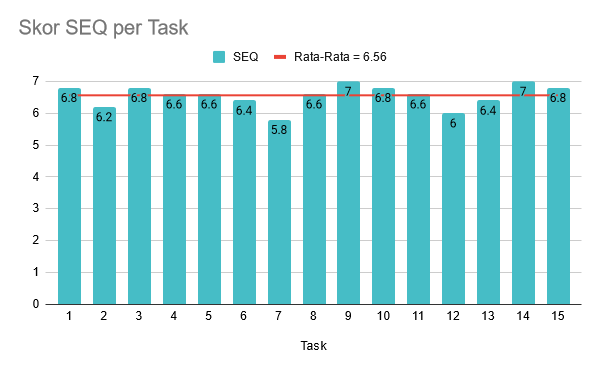
\includegraphics[width=0.6\textwidth]{hifi/hasil-seq.png}
    \caption{Hasil \textit{Single Ease Question} Pengujian Prototipe \textit{High-Fidelity} Iterasi Pertama}
    \label{img:seq_1}
  \end{figure}
  \FloatBarrier

  \item \textit{System Usability Scale} (SUS)
  \subitem  Berdasarkan hasil nilai SUS yang tertera pada Gambar \ref{img:sus_1} terlihat bahwa nilai yang diberikan setiap partisipan pada pengerjaan setiap \textit{task} sudah baik. Namun ditemukan bahwa nilai rata-rata SUS terendah adalah 65. Maka dari itu, desain solusi aplikasi masih perlu diperbaiki dalam prototipe \textit{high-fidelity} iterasi kedua agar dapat mencapai \textit{usability goal efficiency} dengan lebih baik. 

  \begin{figure}[h]
    \centering
    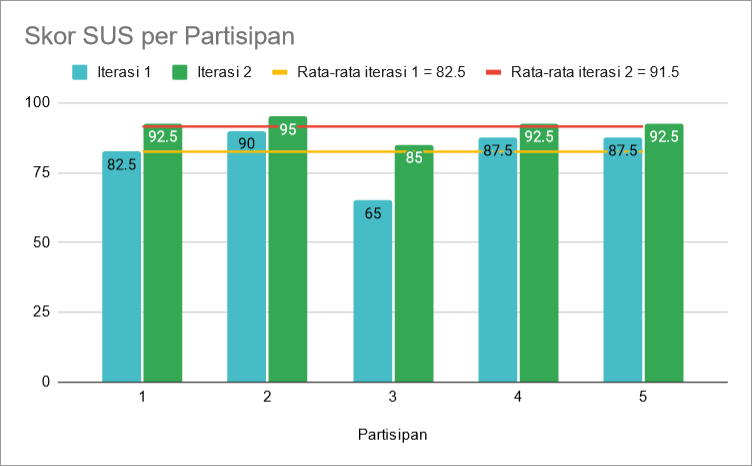
\includegraphics[width=0.6\textwidth]{hifi/hasil-sus.png}
    \caption{Hasil \textit{System Usability Scale} Pengujian Prototipe \textit{High-Fidelity} Iterasi Pertama}
    \label{img:sus_1}
  \end{figure}
  \FloatBarrier

  \item \textit{Intrinsic Motivation Inventory} (IMI)
  \subitem  Berdasarkan Gambar \ref{img:imi1_1} dapat dilihat bahwa skor IMI untuk sub skala \textit{Value/Usefulness} yang didapatkan dari setiap partisipan telah melewati nilai 5 dengan rata-rata skor 6,46. Dengan demikian, rancangan prototipe \textit{high-fidelity} sudah mengarah kepada \textit{user experience goal helpful} dengan baik, namun tetap dibutuhkan beberapa perbaikan yang perlu diperhatikan kembali.
  
  \begin{figure}[h]
    \centering
    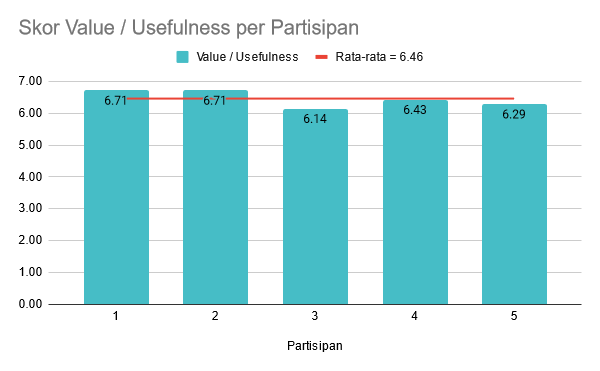
\includegraphics[width=0.6\textwidth]{hifi/hasil-imi1.png}
    \caption{Hasil \textit{Intrinsic Motivation Inventory} Sub Skala \textit{Value/Usefulness} Pengujian Prototipe \textit{High-Fidelity} Iterasi Pertama}
    \label{img:imi1_1}
  \end{figure}
  \FloatBarrier
  
  \subitem  Berdasarkan Gambar \ref{img:imi2_1} dapat dilihat bahwa skor IMI untuk sub skala \textit{Interest/Enjoyment} yang didapatkan dari setiap partisipan telah melewati nilai 5 dengan rata-rata skor 5,69. Di sisi lain, skor IMI untuk sub skala \textit{Pressure/Tension} memiliki nilai rata-rata setelah di-\textit{reverse} yaitu 6,52, yang telah melewati nilai batas 5 juga. Hal tersebut menunjukkan bahwa rancangan prototipe \textit{high-fidelity} sudah cukup mengarah kepada \textit{user experience goal motivating}, dengen perlu perbaikan yang cukup signifikan.

  \begin{figure}[h]
    \centering
    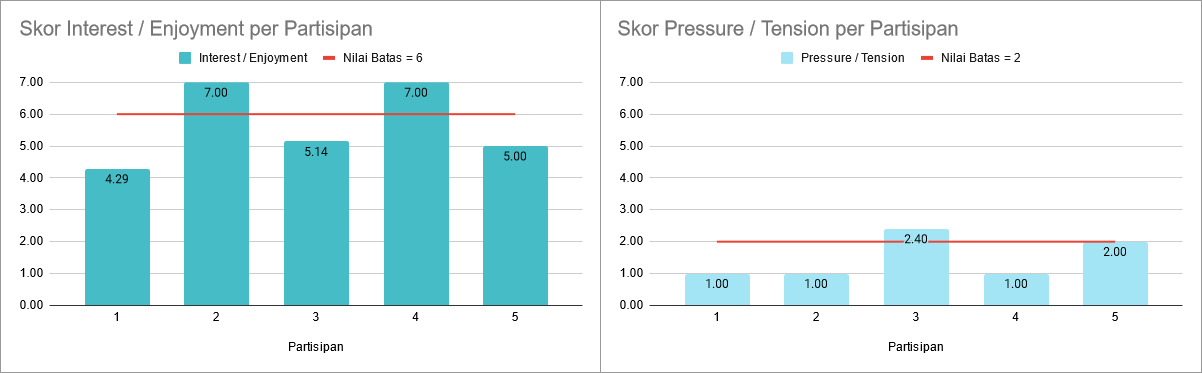
\includegraphics[width=0.9\textwidth]{hifi/hasil-imi2.png}
    \caption{Hasil \textit{Intrinsic Motivation Inventory} Sub Skala \textit{Interest/Enjoyment} dan \textit{Pressure/Tension} Pengujian Prototipe \textit{High-Fidelity} Iterasi Pertama}
    \label{img:imi2_1}
  \end{figure}
  \FloatBarrier

\end{enumerate}




